\section{Rendu: Stratégie et Conception}

\subsection{Stratégie de rendu d'un état}

Nous pouvons diviser notre affichage en deux catégories principales: l'affichage de la carte, et l'affichage des salles.

\textbf{Rendu des salles}

Pour le rendu des salles, nous avons besoin d'afficher trois éléments principaux: des cartes (pour toutes les salles), des joueurs et des ennemis (pour la salle d'ennemis). Nous avons donc décidé de créer une classe "Editeur" afin de créer des textures de ces trois éléments, et une classe "Rendu" dont le rôle est de générer le rendu général de l'affichage.

\underline{Editeur}
\begin{itemize}
    \item int x: position de la texture sur l'axe des abscisses. Cet entier est utilisé afin de positionner la texture pour l'affichage final. Cette position est en pixels.
    \item int y: position de la texture sur l'axe des ordonnées. Cet entier est utilisé afin de positionner la texture pour l'affichage final. Cette position est en pixels.
    \item float scale : l'échelle à appliquer à la texture. Doit être précisée à la création ou à l'édition d'une texture.
    \item sf::RenderTexture : texture correspondant à un joueur/ennemi ou carte. Elle est créée sur un fond transparent.
\end{itemize}

Pour la création de la texture des joueurs et des ennemis, les élements suivants sont à prendre en compte:
\begin{itemize}
    \item Le nom du joueur ou du monstre
    \item Sa vie
    \item Son élément
    \item Ses bonus ou malus, ainsi que le nombre de tours pendant lesquels ils s'appliquent
    \item La valeur de block
    \item L'énergie restante (pour le joueur)
    \item L'intention de l'ennemi (pour l'ennemi), c'est-à-dire une icone représentant l'action qu'il va réaliser, et si c'est une attaque, sa puissance.
\end{itemize}
\newpage
\begin{figure}[h]
\begin{center}
\subfigure{%
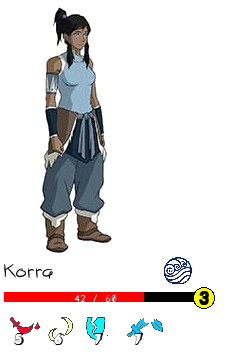
\includegraphics[width=6cm]{images/korra.png}}%
\qquad
\subfigure{%
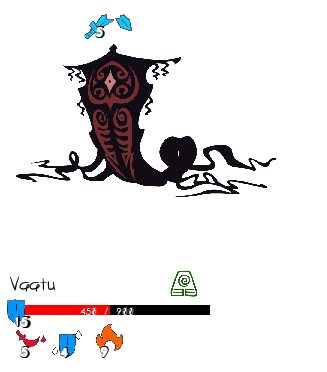
\includegraphics[width=8cm]{images/vaatu.png}}%
\caption{\label{slaythespiregame}Exemple de texture créé pour un joueur (à gauche) et un ennemi (à droite). Au dessus de la barre de vie se situent le nom du personnage ainsi que son élément. Les bonus ou malus sont indiqués en dessous de la barre de vie. La valeur de block pour ce tour est indiquée au côté gauche de la barre de vie, la valeur d'énergie (pour le joueur) est indiquée à droite de la barre de vie. L'intention de l'ennemi est indiquée au dessus de lui.}
\end{center}
\end{figure}

\underline{Rendu}

Le rendu est utilisé afin de générer les différentes textures pour les salles et pour la carte. La classe Rendu utilise des objets de classe Editeur pour ce faire. La création d'une salle consiste en la création de tous les éditeurs nécessaires à la salle et de les placer au bon endroit. Par exemple, une salle d'ennemi aura besoin d'au moins une texture joueur, une texture ennemi, et 7 textures cartes (5 pour la main et 2 pour représenter la pioche et la défausse).

Les attributs de cette classe sont:
\begin{itemize}
\item int dimensionX : un entier indiquant la longueur de la fenêtre à générer en pixels
\item in dimensionY : un entier indiquant la largeur de la fenêtre à générer en pixels.
\item Gamestate * gamestate : un pointeur vers le gamestate.
\end{itemize}

\begin{figure}[H]
\begin{center}
\subfigure{%
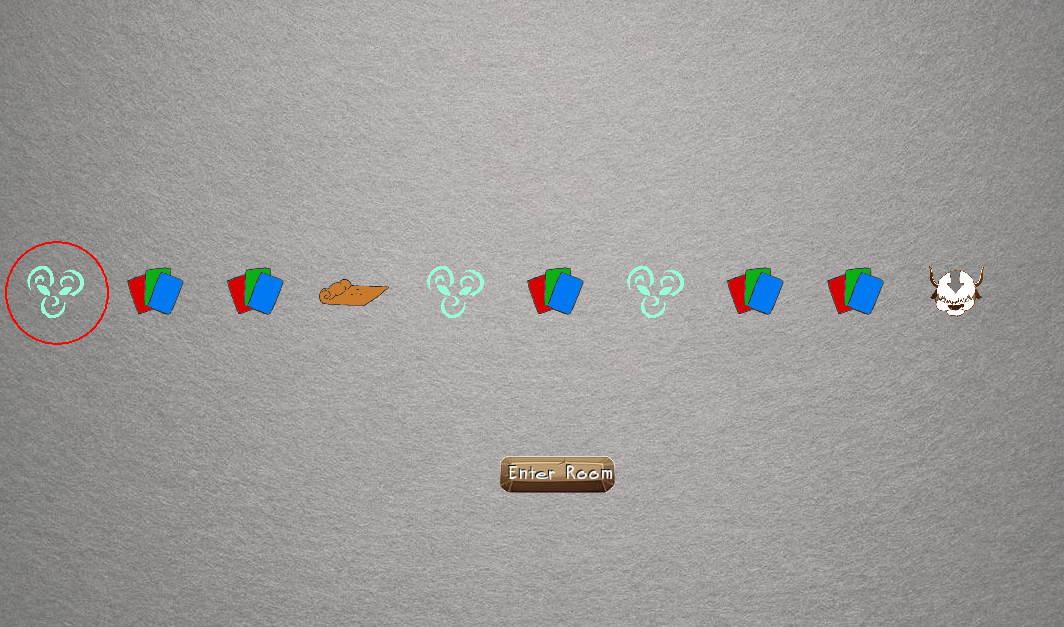
\includegraphics[width=8cm]{images/map_air.png}}%
\qquad
\subfigure{%
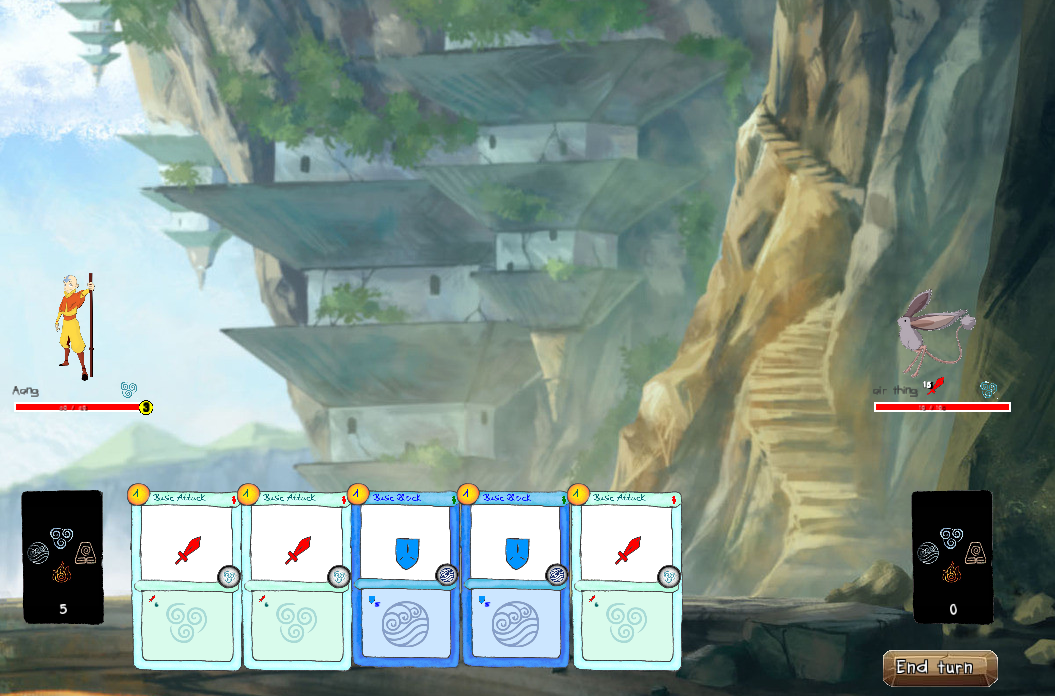
\includegraphics[width=8cm]{images/enemyRoom.png}}%
\qquad
\subfigure{%
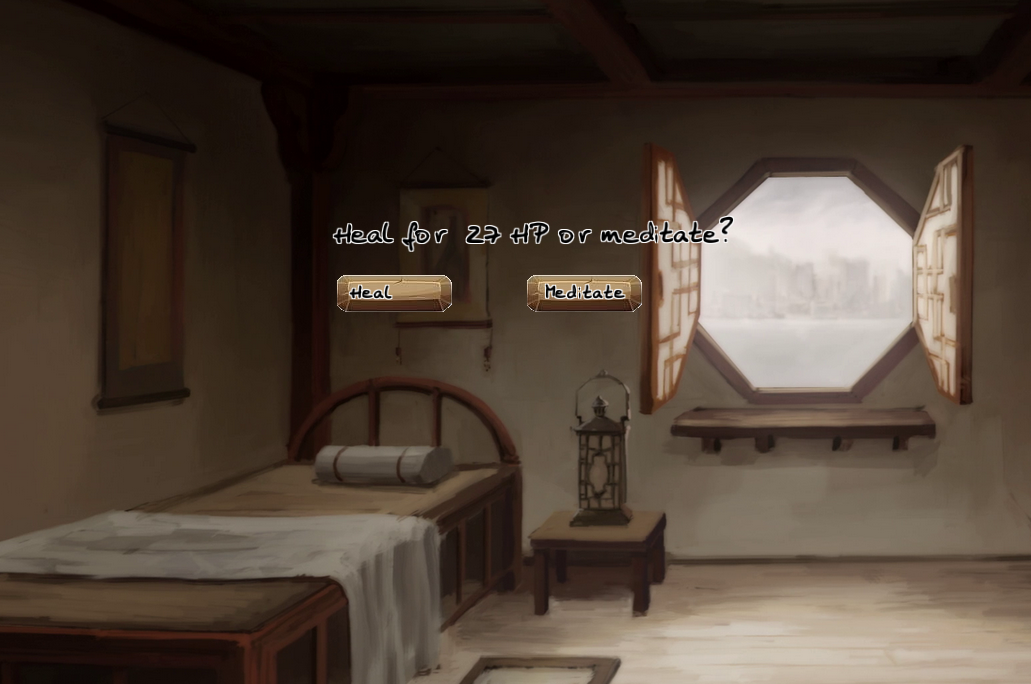
\includegraphics[width=8cm]{images/sleepRoom.png}}%
\qquad
\subfigure{%
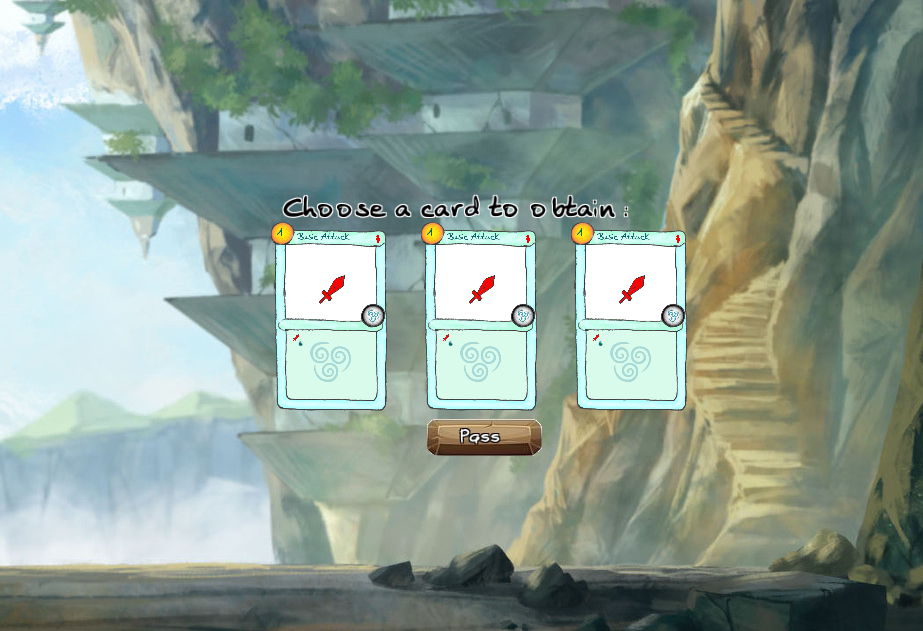
\includegraphics[width=8cm]{images/reward.png}}%
\caption{\label{slaythespiregame}Exemple de rendu final. En haut à gauche la carte, le cercle rouge indique la salle actuelle, en appuyant sur le bouton "enter room" on entre dans la salle. En haut à gauche une salle d'enemis, avec le(s) joueur(s) à gauche, le(s) ennemi(s) à droite, et les cartes du joueur actif en dessous. Les deux cartes au dos noirs indiquent la pioche et la défausse. En bas à gauche une salle de repos, on peut choisir de se soigner ou de méditer pour augmenter ses stats de base. En bas à droite une salle d'entrainement, on peut choisir une carte à ajouter au deck}
\end{center}
\end{figure}

\subsection{Conception logiciel}

L'image qui suit correspond à notre diagramme UML du Rendu d'un état.

\begin{figure}[p]
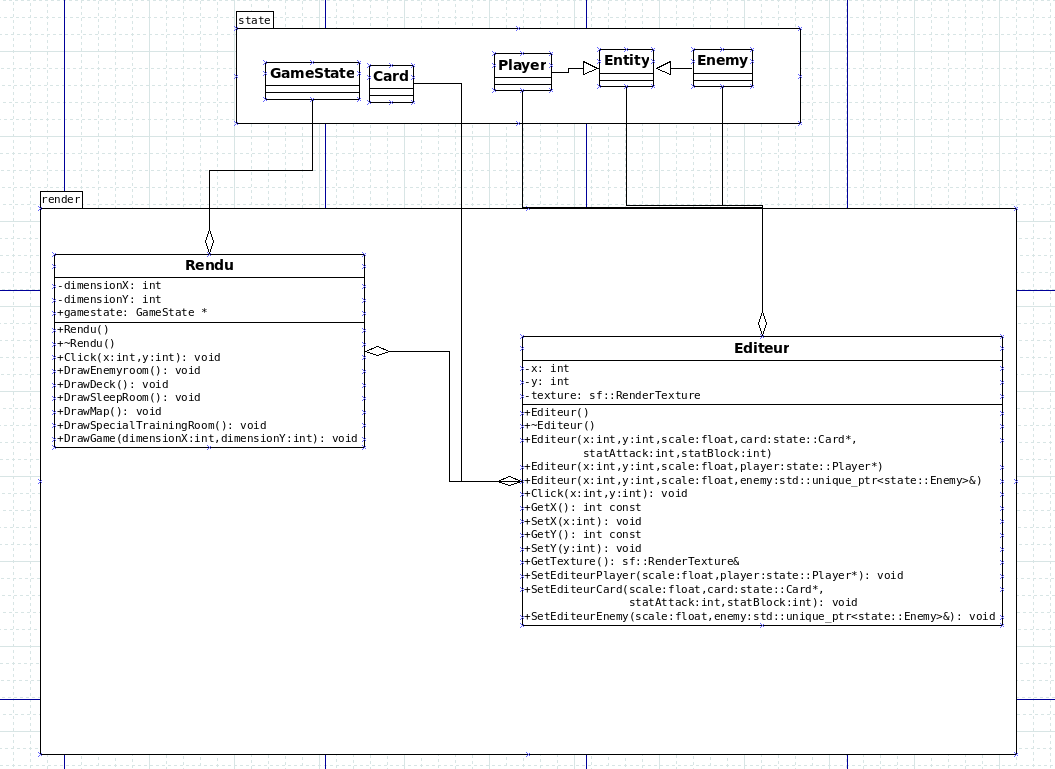
\includegraphics[width = 15cm]{images/render.png}
\caption{\label{uml:render}Diagramme des classes de rendu.} 
\end{figure}


\clearpage